\begin{frame}{\large $d(K^-, n \pi^+ \pi^-)"X"$ tail study by $d(K^-, n)"\pi^{\mp}\Sigma^{\pm}"$ Data dist.}
  \centering
  $n_{forward}$の角度は8度以内に一様分布 \\
  $mass_{\pi\Sigma}$の質量分布はデータを再現する重みを付けてある\\
  $d(K^-, n \pi^+ \pi^-)"n"$への混入は1\%以下 
  \tminipageTwo{
    \begin{figure}
      \scriptsize
      $K^- d\rightarrow \pi^+ \Sigma^- n_{forward}$
      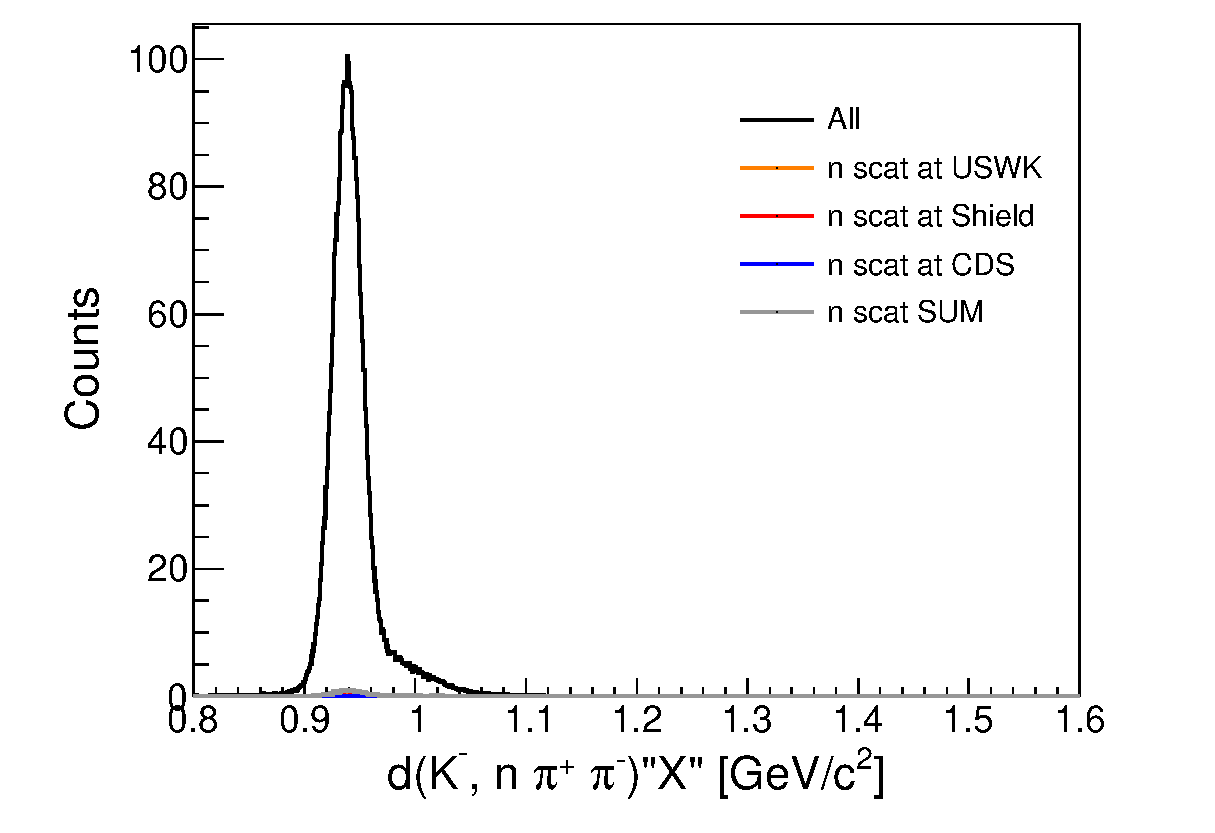
\includegraphics[width=4cm]{../pic/sim/fit_KNpipi_MM_n_scat_nL1405_pipSm.eps}
      \includegraphics[width=4cm]{../pic/sim/fit_KNpipi_MM_n_scat_nL1405_pipSm_logy.eps}
    \end{figure}
  }{
    \begin{figure}
      \scriptsize
      $K^- d\rightarrow \pi^- \Sigma^+ n_{forward}$
      \includegraphics[width=4cm]{../pic/sim/fit_KNpipi_MM_n_scat_nL1405_pimSp.eps}
      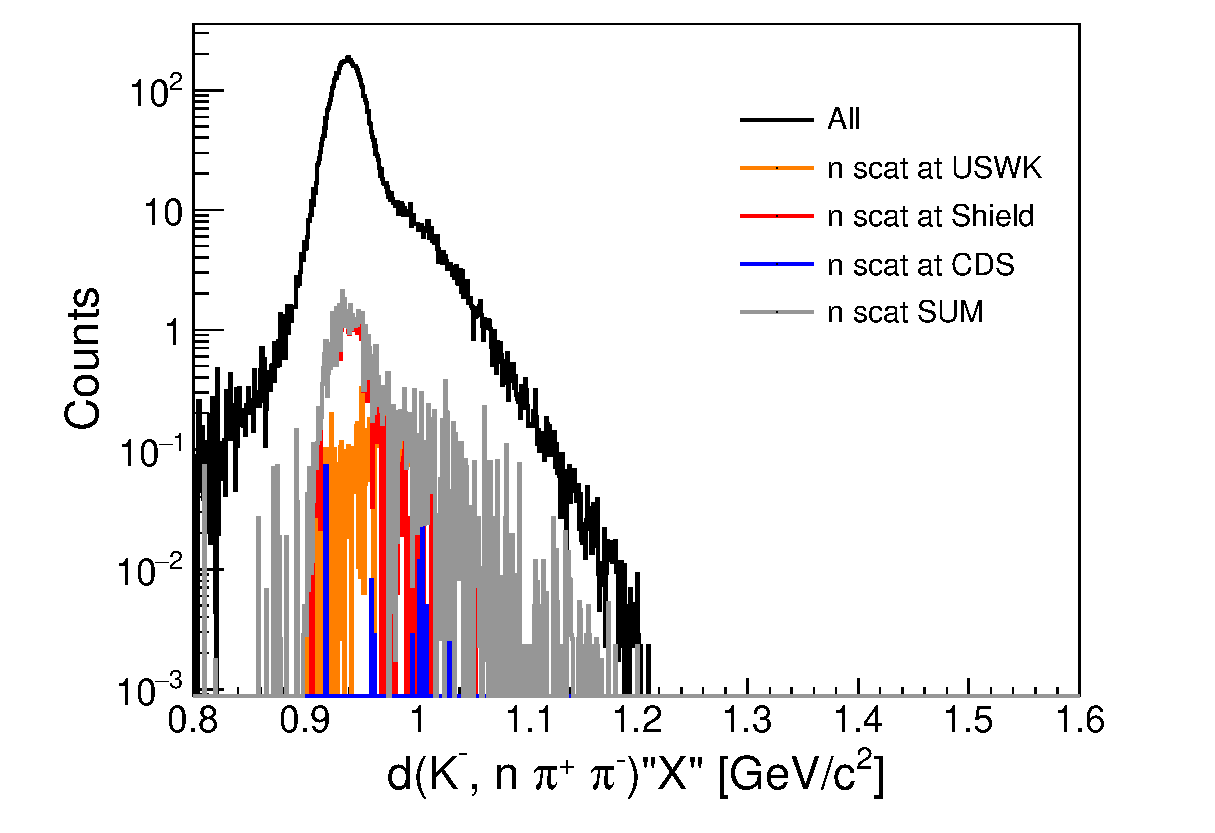
\includegraphics[width=4cm]{../pic/sim/fit_KNpipi_MM_n_scat_nL1405_pimSp_logy.eps}
    \end{figure}
  }
\end{frame}
